\HeaderQuote{It was much pleasanter at home, when one wasn't always growing larger and smaller, and being ordered about by mice and rabbits.}{Alice} 
%\HeaderQuote{The adventures first\dots explanations take such a dreadful time.}{The Gryphon} 

\chapter{Learning Models}\label{ch:prefmodels} \todo[color=green!40,noline]{\cref{ch:prefmodels} Unfinished}

\FirstSentence{L}{earning models considered in this } dissertation are based on ordinal regression in which the learning task is formulated as learning preferences. In the case of scheduling, learning which operations are preferred to others. Ordinal regression has been previously presented in \cite{Ru06:PPSN}, and given in \cref{ch:ordinal} for completeness. 

\section{Ordinal regression for \JSP}

Let $\vphi_{o}\in\R^d$ denote the post-decision state when dispatching $J_o$ corresponds to an optimal schedule being built. All post-decisions states corresponding to suboptimal dispatches, $J_s$, are denoted by $\vphi_{s}\in\R^d$. One could label which feature sets were considered optimal, $\vec{z}_{o}=\vphi_{o}-\vphi_{s}$, and suboptimal, $\vec{z}_{s}=\vphi_{s}-\vphi_{o}$ by $y_o=+1$ and $y_s=-1$ respectively. 
Note, a negative example is only created as long as $J_s$ actually results in a worse makespan, i.e., $C_{\max}^{(s)}\gneq C_{\max}^{(o)}$, since there can exist situations in which more than one operation can be considered optimal.

The preference learning problem is specified by a set of preference pairs,
\begin{equation}
S = \left\{\left\{\vec{z}_o,+1\right\}_{k=1}^{\ell},\left\{\vec{z}_s,-1\right\}_{k=1}^{\ell}
\;|\;\forall (o,s) \in \mathcal{O}^{(k)} \times \mathcal{S}^{(k)}
\right\}\subset \Phi\times Y \label{eq:S:jsp}
\end{equation}
where $\Phi\subset \mathbb{R}^d$ is the training set of $d$ features, $Y=\{-1,+1\}$ is the outcome space, $\ell=n\cdot m$ is the total number of optimal dispatches, $o\in\mathcal{O}^{(k)}$, and suboptimal dispatches $s\in \mathcal{S}^{(k)}$, at dispatch $k$. Note, $\mathcal{O}^{(k)}\cup\mathcal{S}^{(k)}=\mathcal{R}^{(k)}$, and $\mathcal{O}^{(k)}\cap\mathcal{S}^{(k)}=\emptyset$. 

For \JSP\ there are $d=\NrFeatTotal$ features (cf. the step-by-step varying features from \cref{tbl:features}), and the training set is created in the manner described in \cref{sec:gentrainingdata}.

Logistic regression makes decisions regarding optimal dispatches and at the same time efficiently estimates a posteriori probabilities. When using linear classification model (cf. \cref{sec:ord:linpref}), i.e., 
\begin{equation}\label{eq:jssp:linweights}
h(\vec{x})=\sum_{i=1}^d w_i\phi_i(\vec{x})=\inner{\vec{w}}{\vphi(\vec{x})},
\end{equation}
the optimal $\vec{w}^*$ obtained from the preference set can be used on any new data point, $\vphi$, and their inner product is proportional to probability estimate \cref{eq:prob}. 
%Similarly for non-linear classification models. 
Hence, for each job on the ready-list, $J_j\in\mathcal{R}$, let $\vphi_j$ denote its corresponding  post-decision state. Then the job chosen to be dispatched, $J_{j^*}$, is the one corresponding to the highest preference estimate, i.e.,
\begin{equation}\label{eq:lin}
J_{j^*}=\argmax_{J_j\in \mathcal{R}}\; h(\vphi_j)
\end{equation}
where $h(\cdot)$ is the classification model obtained by the preference set, $S$, defined by \cref{eq:S:jsp}. 

\section{Interpreting linear classification models}
Looking at the features description in \cref{tbl:features} it is possible for the ordinal regression to `discover' the weights $\vec{w}$ in order for \cref{eq:jssp:linweights} corresponding applying a single priority dispatching rules from \cref{sec:SDR}. For instance, 
\begin{IEEEeqnarray}{s"rCl}
SPT:& w_i&=&\bigg\{ \begin{array}{rl}-1&\text{if }i=1\\0&\text{otherwise}\end{array} \\
LPT:& w_i&=&\bigg\{ \begin{array}{rl} 1&\text{if }i=1\\0&\text{otherwise}\end{array} \\
MWR:& w_i&=&\bigg\{ \begin{array}{rl} 1&\text{if }i=7\\0&\text{otherwise}\end{array} \\
LWR:& w_i&=&\bigg\{ \begin{array}{rl}-1&\text{if }i=7\\0&\text{otherwise}\end{array}
\end{IEEEeqnarray}
where $i\in\{1,\ldots,d\}$. .
When using a feature space based on single priority dispatching rules, the linear classification models can very easily be interpreted as composite dispatching rules with predetermined weights. 
%Similarly for non-linear classification models, however, they are harder to visualise since the features have to be projected on a kernel.


\section{Generating training data}\label{sec:gentrainingdata} 

For \jsp\ scheduling there are $N$ problem instances generated using $n$ jobs and $m$ machines for processing times following the same data distribution and a random $\sigma$ permutations. 

\subsection{\JSP\ tree representation}\label{sec:gen:gametree}
When building a complete \JSP\ schedule $\ell=n\cdot m$ dispatches must be made sequentially. 
A job is placed at the earliest available time slot for its next machine, whilst still fulfilling constraints \cref{eq:permutation,eq:oneJobPerMac}.
%that each machine can handle at most one job at each time, and jobs need to have finished their previous machines according to its machine order. 
Unfinished jobs are dispatched one at a time according to some heuristic. After each dispatch\footnote{Dispatch and time step are used interchangeably.} the schedule's current features (cf. \cref{tbl:features}) are updated based on the half-finished schedule. \cref{fig:jssp:gametree} shows how the first two dispatches could be executed for a six-job six-machine \jsp\ scheduling problem, with the machines, $a\in\{M_1,...,M_6\}$, on the vertical axis and the horizontal axis yields the current makespan. The next possible dispatches are denoted as dashed boxes with the job index $j$ within and its length corresponding to $p_{ja}$.
In the top layer one can see an empty schedule.
In the middle layer one of the possible dispatches from the layer above is fixed, and one can see the resulting schedule, i.e., what are the next possible dispatches given this scenario? This sort of tree representation is similar to \emph{game trees} \citep[cf.][]{Rosen03} where the root node denotes the initial, i.e., empty, schedule and the leaf nodes denote the complete schedule (resulting after $n\cdot m$ dispatches, thus height of the tree is $\ell$), therefore the distance $k$ from an internal node to the root yields the number of operations already dispatched. Traversing from root to leaf node one can obtain a sequence of dispatches that yielded the resulting schedule, i.e., the sequence indicates in which order the tasks should be dispatched for that particular schedule. 

However one can easily see that this sequence of task assignments is by no means unique. Inspecting a partial schedule further along in the dispatching process such as in \cref{fig:example}, then let's say $J_1$ would be dispatched next, and in the next iteration $J_2$. Now this sequence would yield the same schedule as if $J_2$ would have been dispatched first and then $J_1$ in the next iteration, i.e., these are non-conflicting jobs. Which indicates that some of the nodes in game tree can merge. In the meantime the state of the schedules are different and thus their features, although they manage to yield with the same (partial) schedule at a later date.  % ATHUGASEMD 1 -- SEQ. REP NON-UNIQUE
In this particular instance one can not infer that choosing $J_1$ is better and $J_2$ is worse (or vice versa) since they can both yield the same solution.

Note that in some cases there can be multiple optimal solutions to the same problem instance. Hence not only is the sequence representation `flawed' in the sense that slight permutations on the sequence are in fact equivalent w.r.t. the end-result, but very varying permutations on the dispatching sequence (however given the same partial initial sequence) can result in very different complete schedules but can still achieve the same makespan, and thus same \fullnamerho, which is the measure under consideration. Care must be taken in this case that neither resulting features are labelled as undesirable. Only the resulting features from a dispatch resulting in a suboptimal solution should be labelled undesirable. 

The creation of the game tree for \jsp\ scheduling can be done recursively for all possible permutation of dispatches, in the manner described above, resulting in a full \mbox{$n$-ary} tree (since $|\mathcal{R}|\leq n$) of height $\ell=n\cdot m$. Such an exhaustive search would yield at the most $n^{\ell}$ leaf nodes (worst case scenario being that no sub-trees merge). Now, since the internal vertices, i.e., partial schedules, are only of interest to learn,\footnote{The root is the empty initial schedule and for the last dispatch there is only one option left to dispatch, so there is no preferred `choice' to learn.} the number of those can be at the most \mbox{${}^{n^{\ell}-1}/_{n-1}$}.
Even for small dimensions of $n$ and $m$ the number of internal vertices are quite substantial and thus computationally expensive to investigate them all. Not to mention that this is done iteratively for all $N$ problem instances.

\begin{figure}
%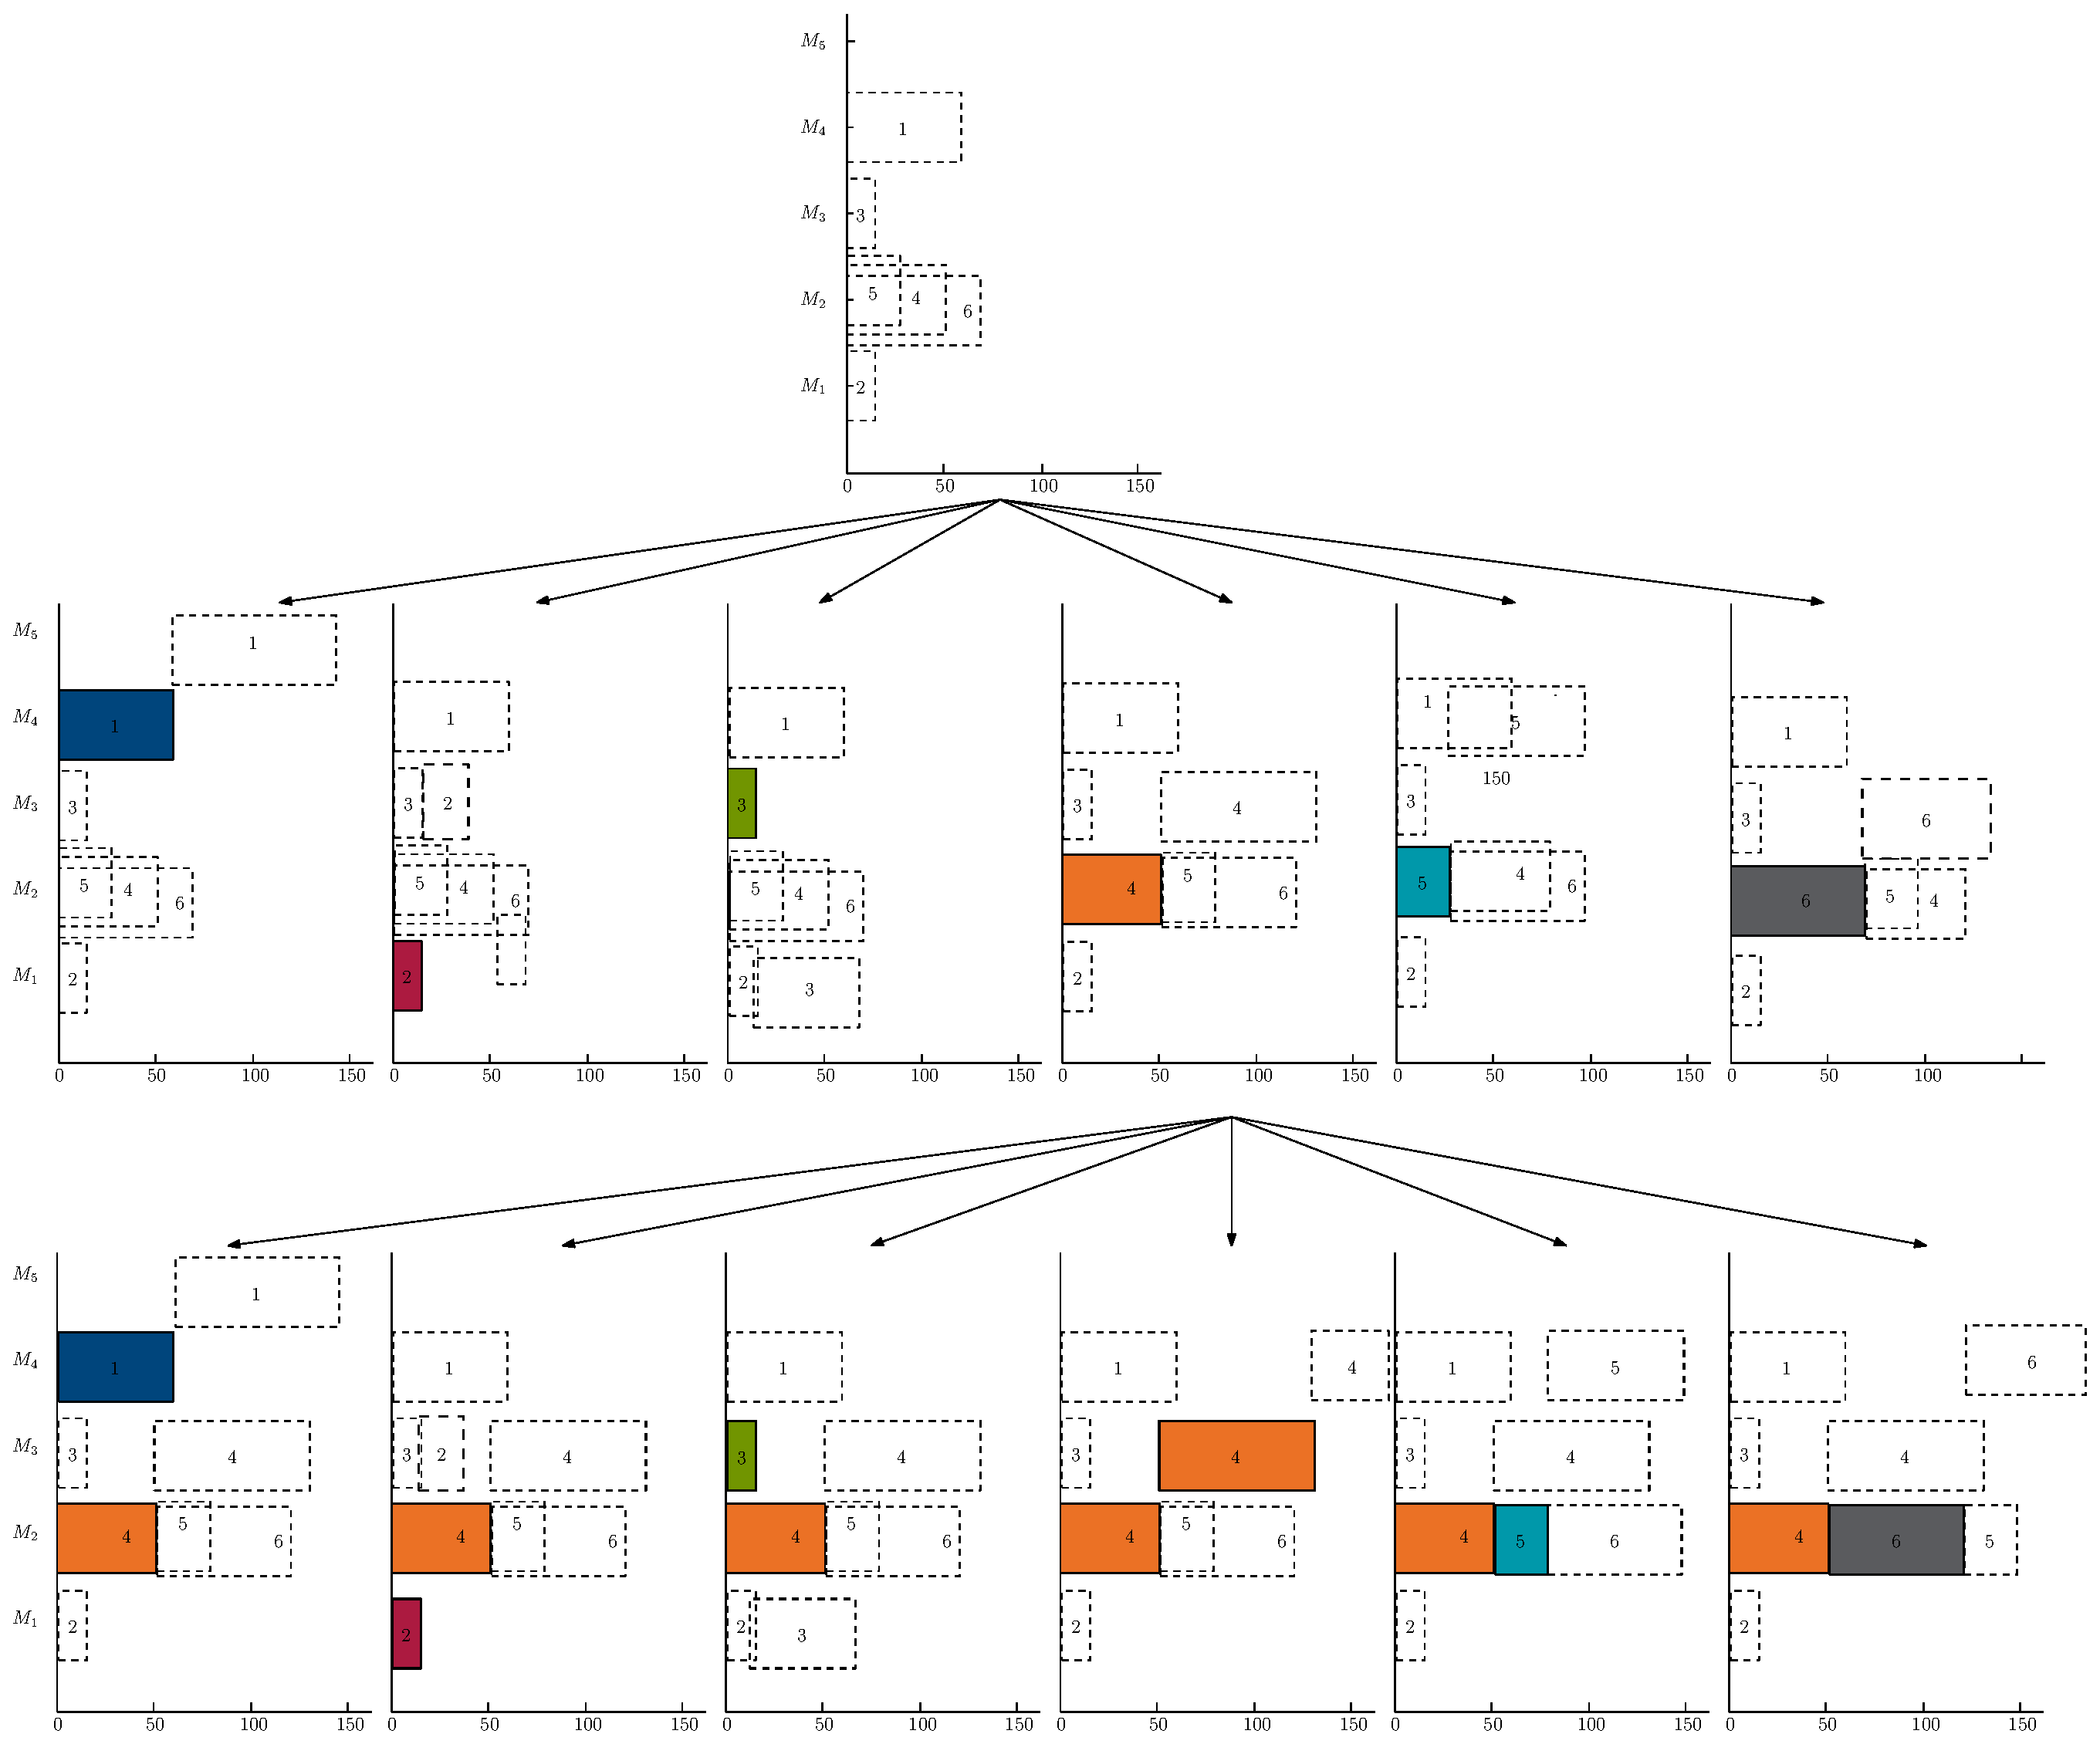
\includegraphics[width=\columnwidth]{gametree}
\caption[Partial Game Tree for \JSP]{Partial Game Tree for \jsp\ scheduling problem for the first two dispatches. 
Top layer depicts all possible dispatches (dashed) for an empty schedule. 
Middle layer depicts all possible dispatches given that one of the dispatches from the layer above has been executed (solid). 
Bottom layer depicts when job $J_3$ on machine $M_4$ has been chosen to be dispatched from the previous layer, moreover it depicts all possible next dispatches from that scenario.}
\label{fig:jssp:gametree}
\end{figure}

\subsection{Labelling schedules w.r.t. optimal decisions}
The optimum makespan is known for each problem instance. 
At each time step (i.e. layer of the game tree) a number of feature pair are created, they consist of the features $\vphi_o$ resulting from optimal dispatches $o\in\mathcal{O}^{(k)}$, versus features $\vphi_s$ resulting from suboptimal dispatches $s\in\mathcal{S}^{(k)}$ at time $k$. Note, $\mathcal{O}^{(k)}\cup\mathcal{S}^{(k)}=\mathcal{R}^{(k)}$ and $\mathcal{O}^{(k)}\cap\mathcal{S}^{(k)}=\emptyset$.
In particular, each job is compared against another job of the ready-list, $\mathcal{R}^{(k)}$, and if the makespan differs, i.e., $C_{\max}^{(s)}\gneq C_{\max}^{(o)}$, an optimal/suboptimal pair is created, however if the makespan would be unaltered the pair is omitted since they give the same optimal makespan. This way, only features from a dispatch resulting in a suboptimal solution is labelled undesirable.

The approach taken here is to verify analytically, at each time step, by fixing the current temporal schedule as an initial state, whether it can indeed \emph{somehow} yield an optimal schedule by manipulating the remainder of the sequence. This also takes care of the scenario that having dispatched a job resulting in a different temporal makespan would have resulted in the same final makespan if another optimal dispatching sequence would have been chosen. That is to say the data generation takes into consideration when there are multiple optimal solutions to the same problem instance. 

\subsection{Selecting preference pairs}\label{sec:S:strategies}
At each dispatch iteration $k$ a number of preference pairs are created which can then be multiplied by the number of problem instance $N$ created. A separate data set is deliberately created for each dispatch iterations, as the initial feeling is that dispatch rules used in the beginning of the schedule building process may not necessarily be the same as in the middle or end of the schedule. As a result there are $\ell$ linear scheduling rules for solving a $n \times m$ \jsp.

Defining the size of the preference set as $l=\abs{S}$, then \cref{eq:S:jsp} gives the size of the feature training set as $\abs{\Phi}=\frac{1}{2}l$. If $l$ is too large, than sampling needs to be done in order for the ordinal regression to be computationally feasible.

Due to the nature of the sequence representation, the earlier stages of the dispatching are more or less equivalent (and thus irrelevant), hence it is appropriate to follow some random optimal path to begin with and then follow some (if not all possible) optimal paths until completion at step $\ell$. The strategy approached in  \cite{InRu11a} was to follow some optimal job $J_j\in\mathcal{O}^{(k)}$, thus creating $\abs{\mathcal{O}^{(k)}}\cdot\abs{\mathcal{S}^{(k)}}$ feature pairs at each dispatch $k$, resulting in a training size of,
\begin{equation}\label{eq:sizeS_b}
l =  \sum_{i=1}^N \left(2 \abs{\mathcal{O}^{(k)}_i}\cdot \abs{\mathcal{S}^{(k)}_i} \right)
\end{equation}
For the data distribution of problem instances considered there, that sort of simple sampling was sufficient for a favourable outcome. However for a considerably harder problem instances (see \cref{ch:genprobleminstances}), preliminary experiments were not to satisfactory. 
A brute force approach was adopted to investigate the feasibility of finding optimal weights $\vec{w}$ for \cref{eq:linearpref}. By applying Covariance Matrix Adaptation Evolution Strategy (CMA-ES) \citep{Hansen01} to minimize the mean $C_{\max}$  w.r.t. the weights $\vec{w}$, gave a considerably more favourable result in predicting optimal versus suboptimal dispatching paths. So the question put forth is, why was the logistic regression not able to detect it?
The nature of the CMA-ES is to explore suboptimal routes until it converges to an optimal one. Implying that the previous approach of only looking into one optimal route is not sufficient information. Which suggest that the training set should incorporate a more complete knowledge about \emph{all} possible preferences, i.e., make also the distinction between suboptimal and sub-suboptimal features, etc.  This would require a Pareto ranking for the ready-list which can be used to make the distinction to which feature sets are equivalent, better or worse -- and to what degree, i.e., by giving a weight to the preference. This would involve a much greater training set, which of course would again need to be sampled in order to be computationally feasible to learn. 

For instance \cite{Siggi05} used decision trees to `rediscover' the LPT single priority based dispatching rule by using the dispatching rule to create its training data. The limitations of using heuristics to label the training data is that the learning algorithm will mimic the original heuristic (both when it works poorly and well on the problem instances) and does not consider the real optimum. In order to learn heuristics that can outperform existing heuristics then the training data needs to be correctly labelled. This drawback is confronted in \citep{Malik08,Russell09,Siggi10} by using an optimal scheduler, computed off-line. 

These aspects are the main motivation for the data generation in this dissertation. All problem instances are correctly labelled; their optimal solution were found using \cite{gurobi}, a commercial software package for solving large-scale linear optimization and a state-of-the-art solver for mixed integer programming. In order to create training instances, i.e., preference pairs, both a features resulting in optimal solutions are gathered (following optimal trajectories) and features that would have been chosen if a dispatching rule had been implemented (following DR trajectories). 
For this dissertation only MWR and LWR will be deemed worthwhile to generate training data, since it is the most promising single priority dispatching rules for \JSP\ and \FSP, respectively, (cf. \cref{ch:problemstructure}).

In conclusion, one needs to consider two main aspects of the generation of the training data, 
\begin{inparaenum}[(a)]
\item What sort of rankings should be compared during each step? 
\item Which path(s) should be investigated? Pursuing solely optimal trajectories? Creating random dispatches? Following other means: CMA-ES computed weights, single priority dispatching rules, etc. 
\end{inparaenum}

\subsubsection{Ranking strategies}
The following ranking strategies were implemented for adding preference pairs to $S$ defined by \cref{eq:S:jsp}, they were first reported in \citet{InRu14b},
\begin{description}
\item[$S_b$] all optimum rankings $r_1$ versus all possible sub-optimum rankings $r_i$, $i\in\{2,\ldots,n'\}$, preference pairs are added, i.e., same basic set-up as in \cite{InRu11a}. Note, $|S_b|$ is defined in \cref{eq:sizeS_b}.
\item[$S_f$] full subsequent rankings, i.e., all possible combinations of $r_i$ and $r_{i+1}$ for $i\in\{1,\ldots,n'\}$, preference pairs are added.
\item[$S_p$] partial subsequent rankings, i.e., sufficient set of combinations of $r_i$ and $r_{i+1}$ for $i\in\{1,\ldots,n'\}$, are added to the training set -- e.g. in the cases that there are more than one operation with the same ranking, only one of that rank is needed to compared to the subsequent rank. Note that $S_p\subset S_f$.
\end{description}
where $r_1>r_2>\ldots>r_{n'}$ ($n'\leq n$) are the rankings of the ready-list, $\mathcal{R}^{(k)}$, at time step $k$.


\subsubsection{Trajectory strategies}
The following trajectory strategies were explored for adding preference pairs to $S$ defined by \cref{eq:S:jsp},
\begin{description}
\item[$S^{opt}$] at each dispatch some (random) optimal task is dispatched.
\item[$S^{cma}$] at each dispatch the task corresponding to highest priority, computed with fixed weights $\vec{w}$, which were obtained by optimising the mean for \fullnamerho, with CMA-ES. 
\item[$S^{mwr}$] at each dispatch the task corresponding to most work remaining is dispatched, i.e., following the simple dispatching rule MWR.
\item[$S^{lwr}$] at each dispatch the task corresponding to most work remaining is dispatched, i.e., following the simple dispatching rule LWR.
\item[$S^{rnd}$] at each dispatch some random task is dispatched.
\end{description}
In the case of $S^{mwr}$ and $S^{cma}$ it is sufficient to explore each trajectory exactly once for each problem instance. Whereas, for $S^{opt}$ and $S^{rnd}$ there can be several trajectories worth exploring, however, only one is chosen (at random). It is noted that since the number of problem instances $N$ is large, it is deemed sufficient to explore one trajectory for each instance, in those cases as well.

These trajectory strategies were initially introduced in \citet{InRu14b}, save for $S^{cma}$ and $S^{lwr}$, however the latter is currently addressed since LWR is considered more favourable for \FSP\ rather than MWR (cf. \cref{ch:problemstructure}). 

\subsection{Experimental study}\label{sec:expr:locallin}
To test the validity of different ranking and strategies from \cref{sec:S:strategies}, a training set of $N_{\text{train}}$ problem instances of $n\times m$ \jsp\ for several problem space distributions, namely problem{1} and problem{2}, described in \cref{tbl:data}. The size of the preference set, $S$, for different trajectory and ranking strategies is depicted in \cref{fig:sizeofprefset:p1} and  \cref{fig:sizeofprefset:p2}, for problem{1} and problem{2}, respectively. 

A linear ordinal regression model (cf. \cref{ch:prefmodels}) was created for each preference set, $S$, for problem space problem{1}. A box-plot with \fullnamerho, is presented in \cref{fig:track:boxplot:p1,fig:rank:boxplot:p2}, note sub-figure (a) uses training data and sub-figure (b) uses test data. \cref{fig:track:boxplot:p1} depicts different ranking strategies for a fixed trajectory, whereas \cref{fig:rank:boxplot:p1} depicts different trajectory strategies for a fixed ranking. 
From the figures it is apparent there can be a performance edge gained by implementing a particular ranking or trajectory strategy, moreover the behaviour is analogous across different disciplines. Similarly, \cref{fig:track:boxplot:p2,fig:rank:boxplot:p2} for problem space problem{2}.


Note that $S_{all}$ denotes that all rankings were explored, i.e., $S_{all}=S_b\cup S_f\cup S_p$. Similarly, $S^{all}=S^{opt}\cup S^{cma}\cup S^{mwr}\cup S^{lwr} \cup S^{rnd}$ for all trajectories.

\missingfigure{Missing plots for different ranking strategies}
\begin{figure}
%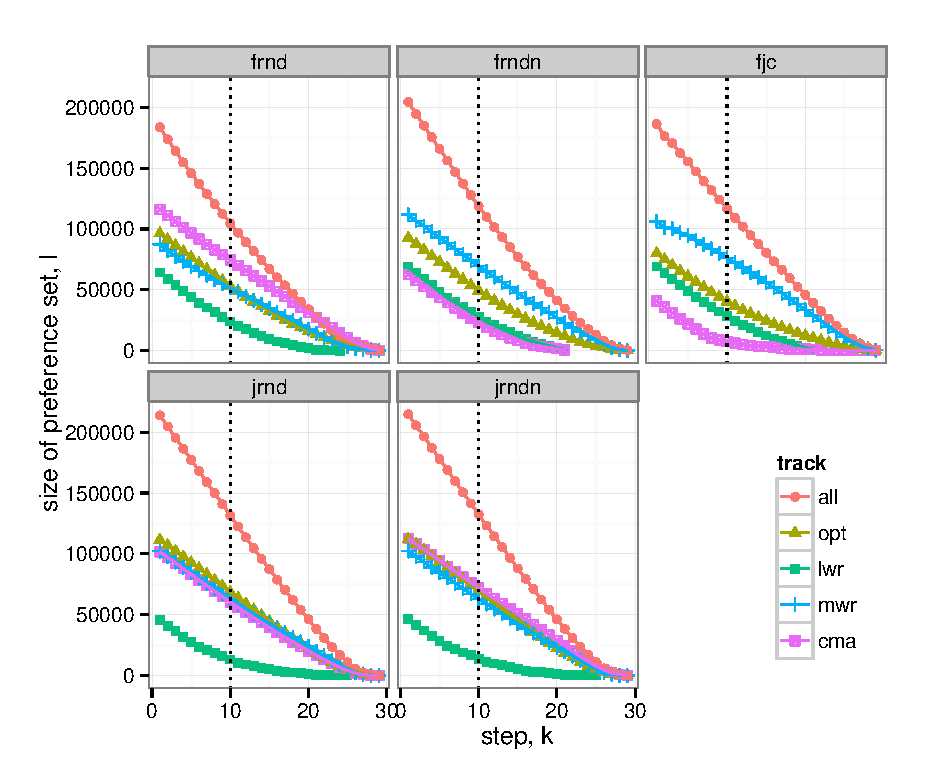
\includegraphics[width=\textwidth]{NUMtrinstances_d30}
\caption{Size of preference set, $l$, for different trajectory strategies for given problem spaces, where $N_{\text{train}}=500$. }
\label{fig:sizeofprefset:p1}
\end{figure}

\todo[inline]{Missing MISTA2013 figures}

\subsubsection{Ranking strategies}
There is no statistical difference between $S_f$ and $S_p$ ranking-schemes across all disciplines (cf. \cref{fig:track:boxplot:p1,fig:track:boxplot:p2}), which is expected since $S_f$ is designed to contain the same preference information as $S_f$. However neither of the Pareto ranking-schemes outperform the original $S_b$ set-up from \cite{InRu11a}. The results hold for the test set as well. 

Combining the ranking schemes, $S_{all}$, improves the individual ranking-schemes across all disciplines, except in the case of $S_b^{opt}\big|_{\mathcal{P_1}}$ and $S_b^{rnd}\big|$\!\Problem{2}, in which case there were no statistical difference. Now, for the test set, the results hold, however there is no statistical difference between $S_b$ and $S_{all}$ for most trajectories $\{S^{opt},S^{cma},S^{rnd}\}\big|$\!\Problem{1} and  $\{S^{opt},S^{rnd}\}\big|$\!\Problem{2}. Now, whereas a smaller preference set is preferred, its opted to use the $S^{b}$ ranking scheme henceforth. 

Moreover, it is noted that the learning algorithm is able to significantly outperform the original heuristics, MWR and CMA-ES (white), used to create the training data $S^{mwr}$ (grey) and $S^{cma}$ (yellow), respectively (cf. \cref{fig:track:boxplot:p1,fig:track:boxplot:p2}). For both \Problem{1} and \Problem{2}, linear ordinal regression models based on $S^{mwr}$ are significantly better than $MWR$, irrespective of the ranking schemes. Whereas the fixed weights found via CMA-ES are only outperformed by linear ordinal regression models based on $\{S_b^{cma},S_{all}^{cma}\}$. This implies that ranking scheme needs to be selected appropriately. Result hold for the test data.

\subsubsection{Trajectory strategies}
Learning preference pairs from a good scheduling policies, such as $S^{cma}$ and $S^{mwr}$, gave considerably more favourable results than tracking optimal paths (cf. \cref{fig:track:boxplot:p1,fig:track:boxplot:p2}). Suboptimal routes are preferred when dealing with problem{1} (for all ranking schemes), however when encountering problem{2} the choice of ranking schemes can yield the exact opposite.

It is particularly interesting there is no statistical difference between $S^{opt}$ and $S^{rnd}$ for both $\{S_{b},S_{f}\}\big|$\Problem{1} and $\{S_b,S_f,S_p\}\big|$\Problem{2} ranking-schemes. That is to say, tracking optimal dispatches gives the same performance as completely random dispatches. This indicates that exploring only optimal trajectories can result in a training set which the learning algorithm is inept to determine good dispatches in the circumstances when newly encountered features have diverged from the learned feature set labelled to optimum solutions. 

Finally, $S^{all}$ gave the best combination across all disciplines. Adding suboptimal trajectories with the optimal trajectories gives the learning algorithm a greater variety of preference pairs for getting out of local minima.

\subsubsection{Following CMA-ES guided trajectory}
The rational for using the $S^{cma}$ strategy was mostly due to the fact a linear classifier is creating the training data (using the weights found via CMA-ES optimisation), hence the training data created should be linearly separable, which in turn should boost the training accuracy for a linear classification learning model. However, this strategy is easily outperformed by the single priority based dispatching rule MWR guiding the training data collection, $S^{mwr}$. 

Let's inspect the CMA-ES guided training data more closely, in particular the linear weights for \cref{eq:jssp:linweights}. The weights are depicted in \cref{fig:weights:p1,fig:weights:p2} for problem space problem{1} and problem{2}, respectively. The original weights found via CMA-ES optimisation, that are used to guide the collection of training data, are depicted in red and  weights obtained by the linear classification model for $S_b^{cma}$ are depicted in blue.


\begin{figure}\centering
%\begin{subfigure}[b]{0.3\textwidth}\includegraphics[width=\textwidth]{weights/p1w1}\caption{$w_1$}\end{subfigure}
%\begin{subfigure}[b]{0.3\textwidth}\includegraphics[width=\textwidth]{weights/p1w2}\caption{$w_2$}\end{subfigure}
%\begin{subfigure}[b]{0.3\textwidth}\includegraphics[width=\textwidth]{weights/p1w3}\caption{$w_3$}\end{subfigure}
%\begin{subfigure}[b]{0.3\textwidth}\includegraphics[width=\textwidth]{weights/p1w4}\caption{$w_4$}\end{subfigure}
%\begin{subfigure}[b]{0.3\textwidth}\includegraphics[width=\textwidth]{weights/p1w5}\caption{$w_5$}\end{subfigure}
%\begin{subfigure}[b]{0.3\textwidth}\includegraphics[width=\textwidth]{weights/p1w6}\caption{$w_6$}\end{subfigure}
%\begin{subfigure}[b]{0.3\textwidth}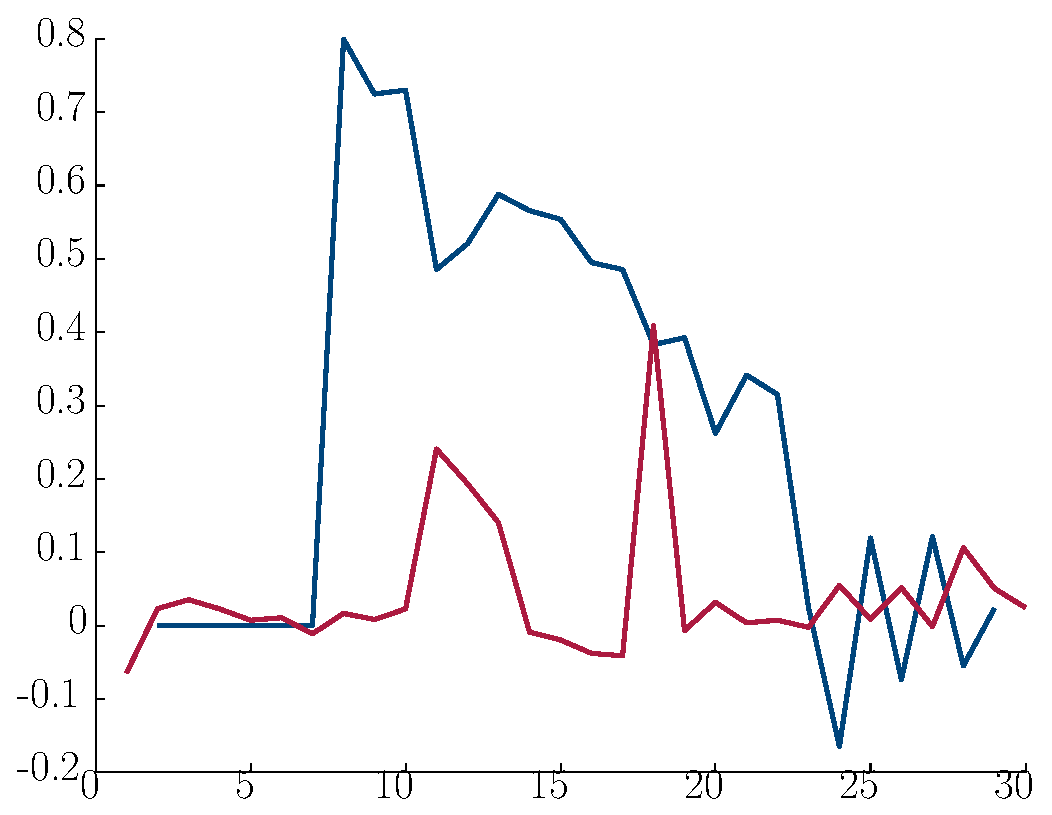
\includegraphics[width=\textwidth]{weights/p1w7}\caption{$w_7$}\end{subfigure}
%\begin{subfigure}[b]{0.3\textwidth}\includegraphics[width=\textwidth]{weights/p1w8}\caption{$w_8$}\end{subfigure}
%\begin{subfigure}[b]{0.3\textwidth}\includegraphics[width=\textwidth]{weights/p1w9}\caption{$w_9$}\end{subfigure}
%\begin{subfigure}[b]{0.3\textwidth}\includegraphics[width=\textwidth]{weights/p1w10}\caption{$w_{10}$}\end{subfigure}
%\begin{subfigure}[b]{0.3\textwidth}\includegraphics[width=\textwidth]{weights/p1w11}\caption{$w_{11}$}\end{subfigure}
%\begin{subfigure}[b]{0.3\textwidth}\includegraphics[width=\textwidth]{weights/p1w12}\caption{$w_{12}$}\end{subfigure}
%\begin{subfigure}[b]{0.3\textwidth}\includegraphics[width=\textwidth]{weights/p1w13}\caption{$w_{13}$}\end{subfigure}
\caption{Linear weights for $\mathcal{P_1}$. Weights found via CMA-ES optimisation (red), and weights found via learning classification model based on $S_b^{cma}$ (blue).}\label{fig:weights:p1}
\end{figure}

\begin{figure}\centering
%\begin{subfigure}[b]{0.3\textwidth}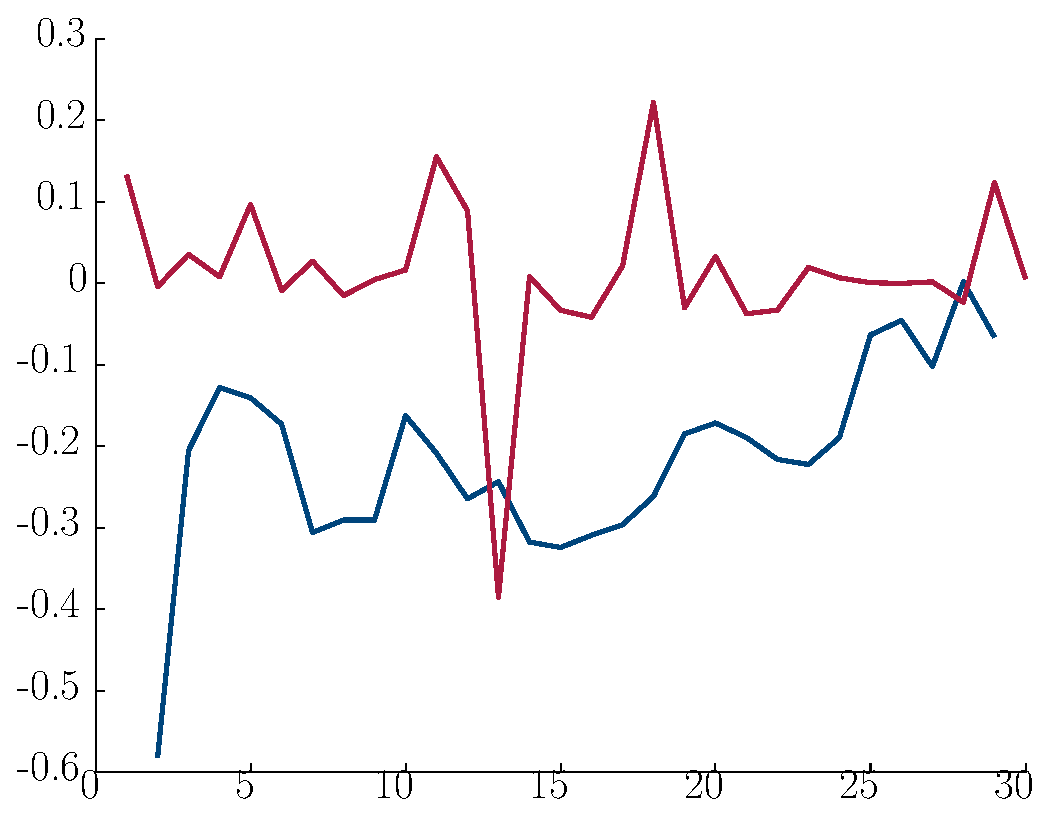
\includegraphics[width=\textwidth]{weights/p2w1}\caption{$w_1$}\end{subfigure}
%\begin{subfigure}[b]{0.3\textwidth}\includegraphics[width=\textwidth]{weights/p2w2}\caption{$w_2$}\end{subfigure}
%\begin{subfigure}[b]{0.3\textwidth}\includegraphics[width=\textwidth]{weights/p2w3}\caption{$w_3$}\end{subfigure}
%\begin{subfigure}[b]{0.3\textwidth}\includegraphics[width=\textwidth]{weights/p2w4}\caption{$w_4$}\end{subfigure}
%\begin{subfigure}[b]{0.3\textwidth}\includegraphics[width=\textwidth]{weights/p2w5}\caption{$w_5$}\end{subfigure}
%\begin{subfigure}[b]{0.3\textwidth}\includegraphics[width=\textwidth]{weights/p2w6}\caption{$w_6$}\end{subfigure}
%\begin{subfigure}[b]{0.3\textwidth}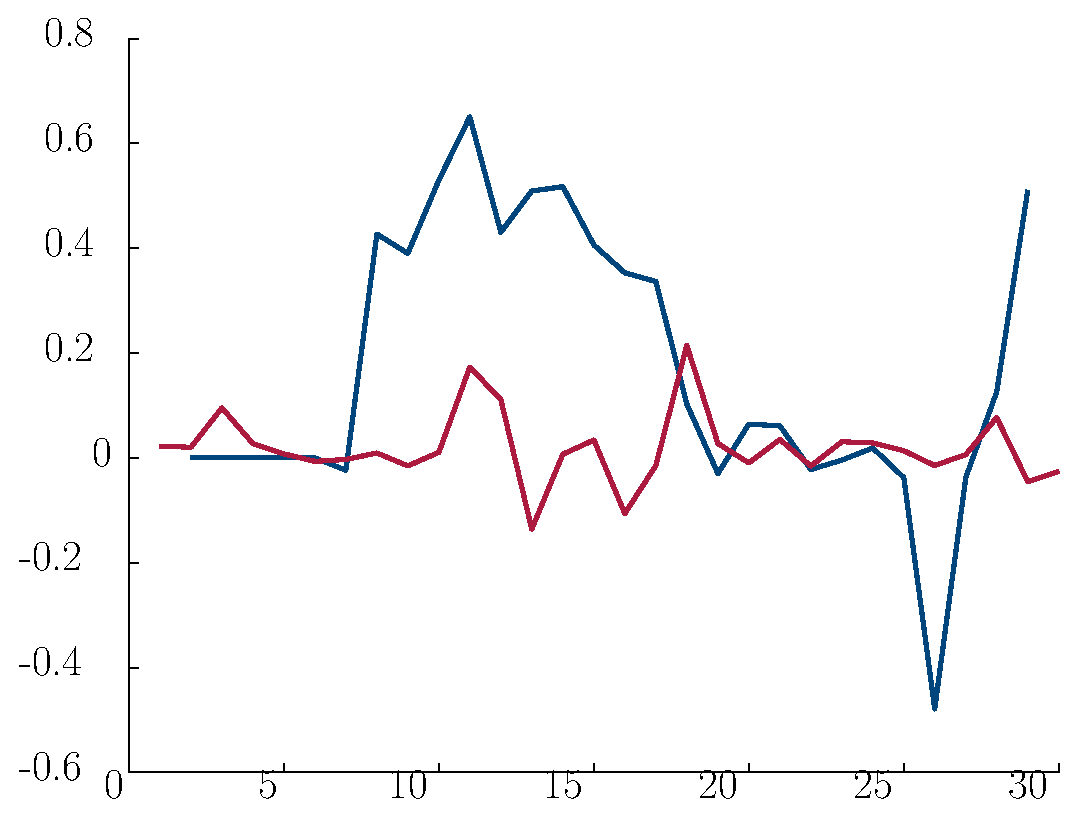
\includegraphics[width=\textwidth]{weights/p2w7}\caption{$w_7$}\end{subfigure}
%\begin{subfigure}[b]{0.3\textwidth}\includegraphics[width=\textwidth]{weights/p2w8}\caption{$w_8$}\end{subfigure}
%\begin{subfigure}[b]{0.3\textwidth}\includegraphics[width=\textwidth]{weights/p2w9}\caption{$w_9$}\end{subfigure}
%\begin{subfigure}[b]{0.3\textwidth}\includegraphics[width=\textwidth]{weights/p2w10}\caption{$w_{10}$}\end{subfigure}
%\begin{subfigure}[b]{0.3\textwidth}\includegraphics[width=\textwidth]{weights/p2w11}\caption{$w_{11}$}\end{subfigure}
%\begin{subfigure}[b]{0.3\textwidth}\includegraphics[width=\textwidth]{weights/p2w12}\caption{$w_{12}$}\end{subfigure}
%\begin{subfigure}[b]{0.3\textwidth}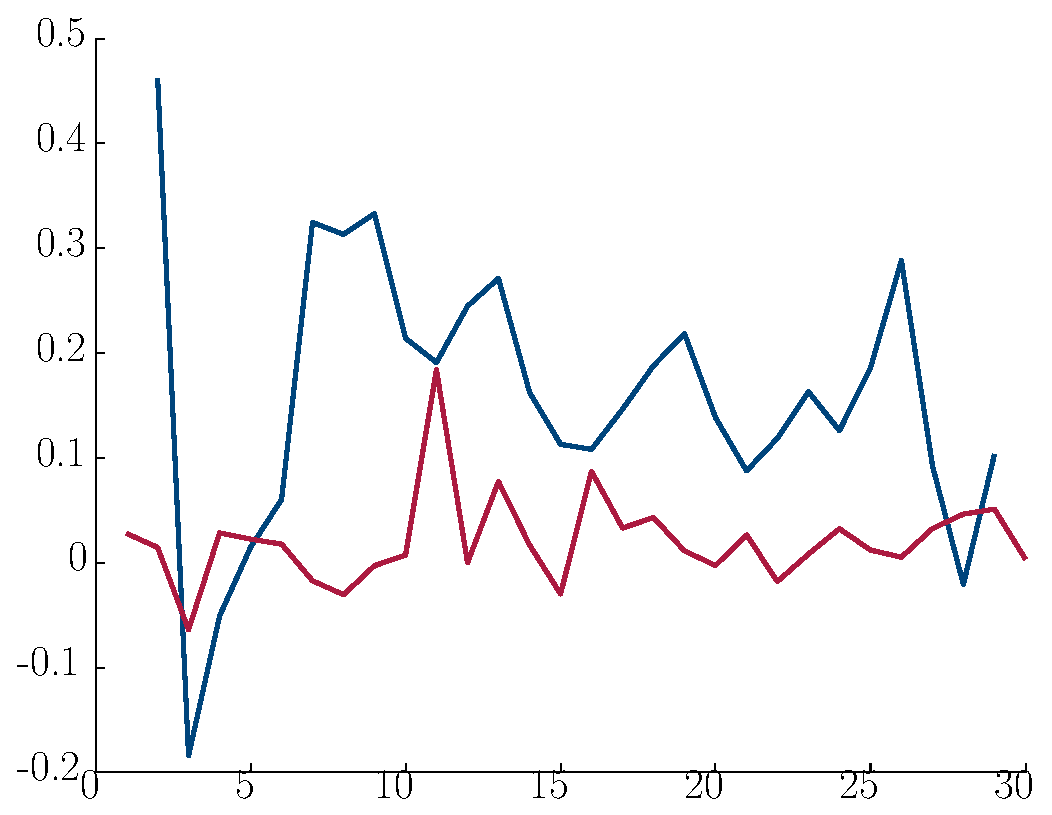
\includegraphics[width=\textwidth]{weights/p2w13}\caption{$w_{13}$}\end{subfigure}
\caption{Linear weights for $\mathcal{P_2}$. Weights found via CMA-ES optimisation in red, and weights found via learning classification model based on $S_b^{cma}$ in blue.}\label{fig:weights:p2}
\end{figure}


\subsubsection{Summary and conclusion }
As the experimental results showed in \cref{sec:expr:locallin}, the ranking of optimal\footnote{Here the tasks labelled `optimal' do not necessarily yield the optimum makespan (except in the case of following optimal trajectories), instead these are the optimal dispatches for the given partial schedule.} and suboptimal features are of paramount importance. The subsequent rankings are not of much value, since they are disregarded anyway. However, the trajectories to create training instances have to be varied.

Unlike \citep{Siggi10,Malik08,Russell09}, learning only on optimal training data was not fruitful. However, inspired by the original work by \cite{Siggi05}, having DR guide the generation of training data (except correctly labelling with analytic means) gave meaningful preference pairs which the learning algorithm could learn. In conclusion, henceforth, the training data will be generate with $S_{b}^{all}$ scheme.

\subsection{Creating time-independent dispatching rules}
As stated in \cref{sec:S:strategies}, a separate data set is deliberately created for each dispatch iteration, as it is initially assumed that dispatch rules used in the schedule building might differ in the beginning, the middle or towards the end of the process. As a result there is a local linear model for each dispatch; a total of $\ell$ linear models for solving $n\times m$ \jsp. Now, if we were to create a global rule, then there would have to be one model for all dispatches iterations. The approach in \cite{InRu11a} was to take the mean weight for all stepwise linear models, i.e., $\bar{w}_i=\frac{1}{\ell}\sum_{k=1}^{\ell}w_i^{(k)}$ where $\vec{w}^{(k)}$ is the linear weight resulting from learning preference set $S^{(k)}$ at dispatch $k$. 

A more sophisticated way, would be to create a \emph{new} linear model, where the preference set, $S$, is the union of the preference pairs across the $\ell$ dispatches. This would amount to a substantial training set, and for $S$ to be computationally feasible to learn, $S$ has to be filtered to size $l_{\max}$.
Now, due to the nature of the sequence representation, earlier dispatches are more or less equivalent (and thus irrelevant) and therefore it is appropriate to follow some random dispatches in the beginning, and then dispatch according to some model. Let's define, $\zeta_k$ as the preference pairs resulting from time step $k$ through $\ell$, i.e., 
\begin{equation}
\zeta_k=\bigcup_{i=k}^{\ell} S^{(k)} \label{eq:zetak}.
\end{equation}

\subsection{Experimental study}\label{sec:global}
Given $N=500$ problem instances of 6-jobs 5-machines \jsp, one can see from \cref{fig:global:sizeofprefset} that $l=|\zeta_k|$ can be quite great for small $k$. Hence, the size of the preference set $\zeta_k$ is limited to $l_{\max}\leq 3.5\times10^{5}$ via random sampling prior implementing the learning algorithm. The training accuracy for the linear ordinal regression model is depicted in \cref{fig:global:tracc}, for problem space distributions problem{1} and problem{2}, described in \cref{tbl:data}.
Moreover, a box-plot for \fullnamerho, for problem spaces considered are depicted in  \cref{fig:stepbystep:boxplot}. Note, figures utilize training set of size $N_{\text{train}}$ in all cases. Main statistics are reported in \cref{tbl:comp:p1p2p3:summary}. 

\begin{figure}\centering 
%\includegraphics[width=0.8\textwidth]{global_numTrainingUnfiltered}
\caption{Size of preference set, $l$, for $\zeta_k$ defined by \cref{eq:zetak}, given $N_{\text{train}}=500$ problem instances for problem spaces problem{1} (blue) and problem{2} (red).}
\label{fig:global:sizeofprefset}
\end{figure}

\begin{figure}\centering
%\includegraphics[width=0.8\textwidth]{global_trainingacc}
\caption{Training accuracy for linear ordinal regression model trained on $\zeta_k$ defined by \cref{eq:zetak}, given $N_{\text{train}}=500$ problem instances for problem spaces problem{1} (blue) and problem{2} (red).}
\label{fig:global:tracc}
\end{figure}

\begin{figure}\centering
%\subfloat[][Training set for $\fjc{6}{5}]{\includegraphics[height=0.8\textheight]{STEPBYSTEPfjc_rp.pdf}}\label{fig:sbs:fjc}
\end{figure}

\begin{figure}\centering
\ContinuedFloat 
%\subfloat[][Training set for \frnd{6}{5}]{\includegraphics[height=0.8\textheight]{STEPBYSTEPfrnd_rp.pdf}}\label{fig:sbs:frnd}
\end{figure}

\begin{figure} \centering
\ContinuedFloat 
%\subfloat[][Training set for \frndn{6}{5}]{\includegraphics[height=0.8\textheight]{STEPBYSTEPfrndn_rp.pdf}}\label{fig:sbs:frndn}
\end{figure}

\begin{figure}\centering
\ContinuedFloat 
%\subfloat[][Training set for \jrnd{6}{5}]{\includegraphics[height=0.8\textheight]{STEPBYSTEPjrnd_rp.pdf}}\label{fig:sbs:jrnd}
\end{figure}

\begin{figure}\centering
\ContinuedFloat 
%\subfloat[][Training set for \jrndn{6}{5}]{\includegraphics[height=0.8\textheight]{STEPBYSTEPjrndn_rp.pdf}}\label{fig:sbs:jrndn}
\caption{Box-plot of results for linear ordinal regression model trained on $\zeta_k$ defined by \cref{eq:zetak}, given $N=1,000$ problem instances for all considered $6\times5$ problem spaces.}\label{fig:stepbystep:boxplot}
\end{figure}

\todo[inline]{Add  $S_b^{all}$ which uses a separate local model for each step $k$, is shown on the far left for comparison  in \cref{fig:stepbystep:boxplot} ?!?}


\begin{figure}\centering
%\begin{subfigure}[b]{0.49\textwidth}\centering
%\subfloat[][Test set, problem{1}]{\includegraphics[width=0.5\textwidth]{global_p1}}\label{fig:global:p1}
%\subfloat[][Test set, problem{2}]{\includegraphics[width=0.5\textwidth]{global_p1}}\label{fig:global:p2}
%\subfloat[][Test set, problem{3}]{\includegraphics[width=0.5\textwidth]{global_p1}}\label{fig:global:p3}
\caption{Box-plot of results for global linear ordinal regression model, $\zeta_{14}$, trained on problem spaces problem{1} (blue) and problem{2} (red). Note, the step-by-step $S_b^{all}$ model for corresponding testing set is shown on the far left for comparison.}
\label{fig:global}
\end{figure}

\begin{table}\centering
\caption{Main statistics for \namerho, using problem spaces \Problem{1}, \Problem{2} and \Problem{3} using several scheduling policies}\label{tbl:comp:p1p2p3:summary}
%\begin{tabular}{c|l|r|rrrrrr|}
\multicolumn{3}{c}{}&\multicolumn{6}{c}{scheduling policies}\\
\cline{4-9}
\multicolumn{2}{c}{}&statistic&LPT&SPT&MWR&LWR&$h_1$&$h_2$\\
\cline{2-9}
\multirow{21}{*}{\begin{sideways}test sets\end{sideways}}
&\multirow{7}{*}{$\mathcal{P}_1$}&min& 3.91& 5.71& {\bf 0.00}& 5.69& {\bf 0.00}& {\bf 0.00} \\
&&2.5th pctl.& 6.57& 12.16& 2.45& 18.75& {\bf 0.00}& {\bf 0.00} \\
&&median& 29.57& 38.20& 16.44& 48.56& {\bf 7.13}& 7.66 \\
&&97.5th pctl.& 63.95& 82.57& 35.85& 90.47& {\bf 21.72}& 22.30 \\
&&max& 79.41& 100.80& 51.76& 118.09& {\bf 27.94}& 32.86 \\
&&mean& 31.67& 40.11& 16.95& 49.67& {\bf 7.82}& 8.49 \\
&&std& 14.15& 16.23& 8.62& 17.37& {\bf 5.77}& 6.04 \\
\cline{2-9}
&\multirow{7}{*}{$\mathcal{P}_2$}&min& 4.27& 4.15& {\bf 0.00}& 10.40& {\bf 0.00}& {\bf 0.00} \\
&&2.5th pctl.& 9.89& 11.70& 2.01& 19.57& {\bf 0.00}& {\bf 0.00} \\
&&median& 29.57& 37.46& 13.78& 44.12& {\bf 7.81}& 8.17 \\
&&97.5th pctl.& 57.29& 70.72& 30.65& 79.07& {\bf 20.25}& 21.11 \\
&&max& 77.32& 95.45& 36.54& 93.63& 26.16& {\bf 24.83 }\\
&&mean& 31.24& 39.04& 14.42& 44.77& {\bf 8.43}& 8.83 \\
&&std& 12.51& 15.33& 7.24& 15.19& {\bf 5.40}& 5.65 \\
\cline{2-9}
&\multirow{7}{*}{$\mathcal{P}_1'$}&min& 14.80& 18.74& 6.55& 25.18&{\bf 2.27}& 2.30 \\
&&2.5th pctl.& 24.01& 28.29& 10.95& 38.52& {\bf 4.99}& 5.78 \\
&&median& 42.81& 48.53& 21.14& 61.51& {\bf 12.40}& 14.42 \\
&&97.5th pctl.& 68.38& 77.52& 34.68& 92.22& {\bf 24.04}& 26.51 \\
&&max& 85.48& 119.28& 43.37& 104.18& {\bf 28.92}& 38.96 \\
&&mean& 43.50& 49.81& 21.33& 62.64& {\bf 13.07}& 14.91 \\
&&std& 11.16& 12.71& 5.96& 14.07& {\bf 4.72}& 5.31 \\
\cline{2-9}
\end{tabular}

\end{table}


%\renewcommand{\arraystretch}{0.8}
\begin{longtable}{|ll|c|r|rrrr|}
\caption{Comparison results of global linear regression model for OR-Library job-shop benchmark problem instances.} \label{tbl:comp:orlibjssp} \\
\hline
\multicolumn{2}{|r|}{Problem space} & Size ($n\times m$) & BKS & \multicolumn{4}{|c|}{Relative deviation from best known solution, $\rho$} \\ \multicolumn{2}{|r|}{} &  & & $\zeta_{15}^{opt}\big|\mathcal{P}_{j,rnd}^{6\times5}$ &
$\zeta_{15}^{all}\big|\mathcal{P}_{j,rnd}^{6\times5}$ &
$\zeta_{15}^{opt}\big|\mathcal{P}_{j,rndn}^{6\times5}$ &
$\zeta_{15}^{all}\big|\mathcal{P}_{j,rndn}^{6\times5}$ \\
\hline
\endfirsthead
\multicolumn{6}{c}%
{\tablename\ \thetable\ -- \textit{Continued from previous page}} \\
\hline
\multicolumn{2}{|r|}{Problem space} & Size ($n\times m$) & BKS & \multicolumn{4}{|c|}{Relative deviation from best known solution, $\rho$} \\ \multicolumn{2}{|r|}{} &  & & $\zeta_{15}^{opt}\big|\mathcal{P}_{j,rnd}^{6\times5}$ &
$\zeta_{15}^{all}\big|\mathcal{P}_{j,rnd}^{6\times5}$ &
$\zeta_{15}^{opt}\big|\mathcal{P}_{j,rndn}^{6\times5}$ &
$\zeta_{15}^{all}\big|\mathcal{P}_{j,rndn}^{6\times5}$ \\ \hline
\endhead
\hline \multicolumn{6}{r}{\textit{Continued on next page}} \\
\endfoot
\hline
\endlastfoot

\multirow{5}{*}{$\mathcal{P}_{abz}$}
& abz5&$10\times10$& 1234 & 14.75 & 10.86 & 12.56 & 61.91\\
& abz6&$10\times10$& 943 & 18.45 & 17.60 & 20.36 & 60.34\\
& abz7&$20\times15$& 731 & 11.49 & 11.35 & 6.84 & 38.85\\
& abz8&$20\times15$& 635 & 51.34 & 27.40 & 36.38 & 76.06\\
& abz9&$20\times15$& 656 & 32.47 & 31.10 & 34.30 & 72.71\\
\hline\pagebreak[2]
\multirow{3}{*}{$\mathcal{P}_{ft}$}
& ft06&$6\times6$& 55 & 18.18 & 10.91 & 14.55 & 36.36\\
& ft10&$10\times10$& 930 & 24.09 & 25.81 & 35.05 & 49.46\\
& ft20&$20\times5$& 1165 & 33.56 & 32.53 & 33.48 & 40.26\\
\hline\pagebreak[2]
\multirow{12}{*}{$\mathcal{P}_{la}$}
& la01&$10\times5$& 666 & 12.76 & 12.76 & 15.47 & 63.66\\
& la02&$10\times5$& 655 & 24.73 & 24.12 & 24.12 & 55.27\\
& la03&$10\times5$& 597 & 24.46 & 22.45 & 16.58 & 50.25\\
& la04&$10\times5$& 590 & 18.81 & 49.83 & 49.83 & 65.25\\
& la05&$10\times5$& 593 & 3.20 & 3.20 & 3.20 & 53.79\\
& la06&$15\times5$& 926 & 3.02 & 3.02 & 3.02 & 22.14\\
& la07&$15\times5$& 890 & 18.20 & 22.58 & 12.47 & 26.97\\
& la08&$15\times5$& 863 & 7.88 & 8.92 & 4.63 & 35.69\\
& la09&$15\times5$& 951 & 8.62 & 8.62 & 8.31 & 44.69\\
& la10&$15\times5$& 958 & 9.50 & 8.25 & 8.25 & 27.45\\
& la11&$20\times5$& 1222 & 7.94 & 5.07 & 4.09 & 44.35\\
& la12&$20\times5$& 1039 & 3.27 & 3.27 & 8.85 & 42.93\\
\multirow{28}{*}{$\mathcal{P}_{la}$} & la13&$20\times5$& 1150 & 4.17 & 4.17 & 5.65 & 42.61\\
& la14&$20\times5$& 1292 & 0.00 & 0.00 & 0.00 & 35.37\\
& la15&$20\times5$& 1207 & 15.82 & 15.16 & 13.17 & 49.46\\
& la16&$10\times10$& 945 & 19.26 & 26.35 & 24.34 & 64.23\\
& la17&$10\times10$& 784 & 17.73 & 19.01 & 14.92 & 85.71\\
& la18&$10\times10$& 848 & 20.52 & 27.95 & 27.24 & 37.03\\
& la19&$10\times10$& 842 & 16.86 & 18.65 & 24.82 & 51.78\\
& la20&$10\times10$& 902 & 24.94 & 16.85 & 20.51 & 81.04\\
& la21&$15\times10$& 1046 & 20.36 & 16.92 & 21.99 & 63.77\\
& la22&$15\times10$& 927 & 24.81 & 22.33 & 27.08 & 50.92\\
& la23&$15\times10$& 1032 & 18.31 & 19.96 & 11.72 & 72.48\\
& la24&$15\times10$& 935 & 25.56 & 22.78 & 27.27 & 39.68\\
& la25&$15\times10$& 977 & 25.79 & 25.38 & 19.96 & 68.58\\
& la26&$20\times10$& 1218 & 15.60 & 17.65 & 14.37 & 55.34\\
& la27&$20\times10$& 1235 & 24.21 & 23.81 & 28.18 & 69.31\\
& la28&$20\times10$& 1216 & 26.56 & 26.56 & 30.59 & 63.16\\
& la29&$20\times10$& 1152 & 29.25 & 22.57 & 27.78 & 61.02\\
& la30&$20\times10$& 1355 & 24.28 & 13.80 & 18.23 & 52.77\\
& la31&$30\times10$& 1784 & 10.20 & 9.36 & 11.15 & 44.45\\
& la32&$30\times10$& 1850 & 8.16 & 4.70 & 4.11 & 51.62\\
& la33&$30\times10$& 1719 & 11.93 & 16.23 & 9.48 & 43.11\\
& la34&$30\times10$& 1721 & 14.06 & 14.06 & 13.89 & 48.75\\
& la35&$30\times10$& 1888 & 8.69 & 9.59 & 16.26 & 30.14\\
& la36&$15\times15$& 1268 & 21.37 & 17.27 & 17.51 & 63.56\\
& la37&$15\times15$& 1397 & 17.82 & 19.97 & 17.68 & 51.54\\
& la38&$15\times15$& 1196 & 36.71 & 27.84 & 21.24 & 77.51\\
& la39&$15\times15$& 1233 & 35.77 & 23.36 & 23.11 & 55.15\\
& la40&$15\times15$& 1222 & 32.82 & 29.79 & 32.41 & 81.42\\
\hline\pagebreak[2]
\multirow{10}{*}{$\mathcal{P}_{orb}$}
& orb01&$10\times10$& 1059 & 36.64 & 28.61 & 36.92 & 28.23\\
& orb02&$10\times10$& 888 & 17.68 & 18.58 & 27.14 & 47.41\\
& orb03&$10\times10$& 1005 & 27.06 & 21.39 & 29.35 & 37.11\\
& orb04&$10\times10$& 1005 & 33.23 & 24.98 & 25.37 & 50.45\\
& orb05&$10\times10$& 887 & 27.62 & 32.58 & 32.24 & 40.59\\
& orb06&$10\times10$& 1010 & 36.53 & 32.77 & 39.60 & 42.97\\
& orb07&$10\times10$& 397 & 31.49 & 17.13 & 24.18 & 52.14\\
& orb08&$10\times10$& 899 & 38.93 & 41.16 & 41.38 & 75.31\\
& orb09&$10\times10$& 934 & 47.54 & 37.79 & 31.05 & 68.63\\
& orb10&$10\times10$& 944 & 39.94 & 34.96 & 29.24 & 52.12\\
\hline\pagebreak[2]
\multirow{4}{*}{$\mathcal{P}_{yn}$}
& yn1&$20\times20$& 888 & 22.30 & 14.64 & 23.09 & 51.69\\
& yn2&$20\times20$& 909 & 35.31 & 19.36 & 21.78 & 78.55\\
& yn3&$20\times20$& 893 & 19.71 & 24.41 & 24.19 & 70.32\\
& yn4&$20\times20$& 968 & 29.96 & 31.71 & 30.89 & 56.82\\
\end{longtable}
\renewcommand{\arraystretch}{1}

\clearpage
\begin{table}\centering
\caption{Main statistics for \namerho, for OR-Library \jsp\ benchmark problem instances using linear ordinal regression scheduling policies}\label{tbl:comp:orlibjssp:summary}
%\begin{tabular}{|l|rrrr|rrrr|} \hline 
Problem space & 
\multicolumn{4}{c|}{$\zeta_{15}\big|\mathcal{P}_{j,rnd}^{opt}$} & \multicolumn{4}{c|}{$\zeta_{15}\big|\mathcal{P}_{j,rnd}^{all}$} \\
&$\min$&mean&$\max$&std&$\min$&mean&$\max$&std\\ \hline
$\mathcal{P}_{abz}$&11.49&25.70&51.34&16.41 &10.86&19.66&31.10&9.24\\
$\mathcal{P}_{ft}$&18.18&25.28&33.56&7.76  &10.91&23.08&32.53&11.07\\
$\mathcal{P}_{la}$&0.00&17.35&36.71&9.26  &0.00&17.10&49.83&9.78\\
$\mathcal{P}_{orb}$&17.68&33.67&47.54&8.28  &17.13&29.00&41.16&8.24\\
$\mathcal{P}_{yn}$&19.71&26.82&35.31&7.14  &14.64&22.53&31.71&7.31\\ \hline\hline
Problem space & 
\multicolumn{4}{c|}{$\zeta_{15}\big|\mathcal{P}_{j,rndn}^{opt}$}& \multicolumn{4}{c|}{$\zeta_{15}\big|\mathcal{P}_{j,rndn}^{all}$}\\
&$\min$&mean&$\max$&std&$\min$&mean&$\max$&std\\ \hline
$\mathcal{P}_{abz}$&6.84&22.09&36.38&13.03 &38.85&61.98&76.06&14.59\\
$\mathcal{P}_{ft}$&14.55&27.69&35.05&11.41  &36.36&42.03&49.46&6.73\\
$\mathcal{P}_{la}$&0.00&17.09&49.83&10.14  &22.14&53.10&85.71&15.50\\
$\mathcal{P}_{orb}$&24.18&31.65&41.38&5.90  &28.23&49.50&75.31&14.06\\
$\mathcal{P}_{yn}$&21.78&24.99&30.89&4.06  &51.69&64.34&78.55&12.31\\
\hline
\end{tabular}

\end{table}

In addition, the global linear regression schedule policies $\zeta_{14}(\mathcal{P}_1)$ and $\zeta_{14}(\mathcal{P}_2)$ were tested on synthetic \FSP\ problems subclasses \frnd{6}{5}, \frndn{6}{5},\fjc{6}{5}, \fmc{6}{5} and \fmxc{6}{5} generated by \citet{Whitley} (cf. \cref{sec:data:FSP}). 

%\clearpage
\renewcommand{\arraystretch}{0.8}
\begin{longtable}{|ll|c|rrr|}
\caption{Comparison results of global linear regression model for OR-Library flow-shop problem instances,   $\mathcal{P}_{for}$.} \label{tbl:comp:orlibfssp}\\
\hline
\multicolumn{2}{|r|}{Problem space} & Size ($n\times m$) & BKS & $\zeta_{14}(\mathcal{P}_1)$ & $\zeta_{14}(\mathcal{P}_2)$ \\
\hline
\endfirsthead
\multicolumn{6}{c}%
{\tablename\ \thetable\ -- \textit{Continued from previous page}} \\
\hline
\multicolumn{2}{|r|}{Problem space} & Size ($n\times m$) & BKS & $\zeta_{14}(\mathcal{P}_1)$ & $\zeta_{14}(\mathcal{P}_2)$ \\
\hline
\endhead
\hline \multicolumn{6}{r}{\textit{Continued on next page}} \\
\endfoot
\hline
\endlastfoot

\multirow{8}{*}{$\mathcal{P}_{car}$}
& car1&$11\times5$&7038&8303&8243\\
& car2&$13\times4$&7166&8640&8759\\
& car3&$12\times5$&7312&8635&8631\\
& car4&$14\times4$&&8956&9645\\
& car5&$10\times6$&&9172&8786\\
& car6&$8\times9$&&9979&10276\\
& car7&$7\times7$&&7390&8182\\
& car8&$8\times8$&&9286&9286\\
\hline\pagebreak[2]
\multirow{2}{*}{$\mathcal{P}_{hel}$}
& hel1&$100\times10$&&528&558\\
& hel2&$20\times10$&&155&164\\
\hline\pagebreak[2]
\multirow{21}{*}{$\mathcal{P}_{rec}$}
& rec01&$20\times5$&&1383&1396\\
& rec03&$20\times5$&&1247&1322\\
& rec05&$20\times5$&&1336&1357\\
& rec07&$20\times10$&&1871&1866\\
& rec09&$20\times10$&&1753&1781\\
& rec11&$20\times10$&&1650&1662\\
& rec13&$20\times15$&&2323&2365\\
& rec15&$20\times15$&&2238&2319\\
& rec17&$20\times15$&&2399&2316\\
& rec19&$30\times10$&&2559&2451\\
& rec21&$30\times10$&&2351&2396\\
& rec23&$30\times10$&&2294&2376\\
& rec25&$30\times15$&&3156&3122\\
& rec27&$30\times15$&&2800&2819\\
& rec29&$30\times15$&&2880&2912\\
& rec31&$50\times10$&&3694&3644\\
& rec33&$50\times10$&&3788&3735\\
& rec35&$50\times10$&&3726&3842\\
& rec37&$75\times20$&&5990&5963\\
& rec39&$75\times20$&&6204&6301\\
& rec41&$75\times20$&&6121&6065\\
\end{longtable}
\renewcommand{\arraystretch}{1} 
%\begin{table}\centering
%\caption{Main statistics for \namerho, for OR-Library \fsp\ benchmark problem instances using linear ordinal regression scheduling policies}
%\begin{tabular}{|ll|rrrr|rrrr|} \hline 
\multicolumn{2}{|c|}{Problem space} & \multicolumn{4}{c|}{$\zeta_{14}(\mathcal{P}_1)$} & \multicolumn{4}{c|}{$\zeta_{14}(\mathcal{P}_2)$}\\
$\quad$&&$\min$&mean&$\max$&std&$\min$&mean&$\max$&std\\ \hline
&$\mathcal{P}_{car}$&&&&&&&& \\
&$\mathcal{P}_{hel} $&&&&&&&& \\
&$\mathcal{P}_{rec} $&&&&&&&& \\
\hline
\end{tabular}

%\end{table}

